\documentclass[a4paper]{article}

\usepackage[english]{babel}
\usepackage[utf8x]{inputenc}
\usepackage{amsmath}
\usepackage{graphicx}
\usepackage{cleveref}
\usepackage{mathtools}
\usepackage{fancyhdr}
\numberwithin{equation}{subsection}
\usepackage[colorinlistoftodos]{todonotes}
 
\newtheorem{theorem}{Theorem}[section]
\newtheorem{corollary}{Corollary}[theorem]
\newtheorem{lemma}[theorem]{Lemma}
\newtheorem{definition}{Definition}[section]

\fancyhf{}
\fancyhead[LE,RO]{\thepage}
\fancyhead[CE]{\Author}
\fancyhead[CO]{\Title}
\renewcommand\headrulewidth{0pt}
\pagestyle{fancy}

\author{Emil Kerimov}
%\title{Basic Trig Functions}

\makeatletter
\let\Title\@author

\begin{document}
\section{PascalRowSum}\label{PascalRowSum}


Prove that:

$${n \choose 0} + {n \choose 1} +
{n \choose 2}+...+{n \choose n} =2^n$$


Draw Pascal's Triangle. 

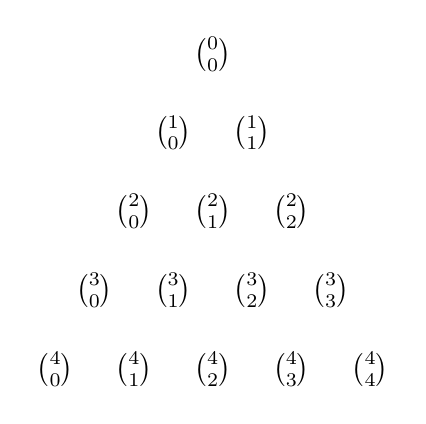
\begin{tikzpicture}
\foreach \n in {0,...,4} {
  \foreach \k in {0,...,\n} {
    \node at (\k-\n/2,-\n) {${\n \choose \k}$};
  }
}
\end{tikzpicture}

Notice, the sum of the nth row seems to be $2^n$.


\subsubsection{Sidenote 1}\label{pascal_sidenote1}
Prove that $${p \choose 0}={p+1 \choose 0}$$
Proof:
$${p \choose 0}=\frac{p!}{0! \cdot (p-0)!}=\frac{p!}{p!}=1=\frac{(p+1)!}{0! \cdot (p+1-0)!}={p+1 \choose 0}$$

\subsubsection{Sidenote 2 }\label{pascal_sidenote2}
Prove that $${p \choose p}={p+1 \choose p+1}$$

Proof:
$${p \choose p}=\frac{p!}{0! \cdot (p-0)!}=\frac{p!}{p!}=1=\frac{(p+1)!}{0! \cdot (p+1-0)!}={p+1 \choose p+1}$$

\subsubsection{Sidenote 3 }\label{pascal_sidenote3}
Prove that $${p \choose q} +{p \choose q+1}={p+1 \choose q+1}$$

Proof:
$${p \choose q} +{p \choose q+1}=\frac{p!}{q! \cdot (p-q)!}+\frac{p!}{(q+1)! \cdot (p-q-1)!} $$
$$=\frac{p! \cdot (q+1)}{(q+1)! \cdot (p-q)!}+\frac{p! \cdot (p-q)}{(q+1)! \cdot (p-q)!} $$
$$= \frac{p! \cdot (q+1+p-q)}{(q+1)! \cdot (p-q)!} = \frac{p! \cdot (p+1)}{(q+1)! \cdot (p-q)!}$$
$$=\frac{(p+1)!}{(q+1)! \cdot (p-q)!}={p+1 \choose q+1} $$


Using induction: 

for n=0:
$${0 \choose 0} = \frac{0!}{0! \cdot 0!}=1=2^0$$

Assume n=k works:
$${k \choose 0} + {k \choose 1} +
{k \choose 2}+...+{k \choose k-2}+{k \choose k-1}+{k \choose k} =2^k$$
Prove for n=k+1
$${k+1 \choose 0} + {k+1 \choose 1} +
{k+1 \choose 2}+...+{k+1 \choose k-1}+{k+1 \choose k}+{k+1 \choose k+1}$$

Using sidenote 1, replace ${k+1 \choose 0}$ with ${k \choose 0}$\\

Using sidenote 2, replace ${k+1 \choose k+1}$ with ${k \choose k}$\\

Using sidenote 2, replace ${k+1 \choose q+1}$ with ${k \choose q} +{k \choose q+1}$\\

$$={k \choose 0} + {k \choose 0}+ {k \choose 1} + {k \choose 1}+ {k \choose 2}+...+{k \choose k-2}+{k \choose k-1}+{k \choose k-1}+{k \choose k}+{k \choose k}$$
$$=2 \cdot ({k \choose 0} + {k \choose 1} +
{k \choose 2}+...+{k \choose k-2}+{k \choose k-1}+{k \choose k}) =2 \cdot (2^k)= 2^{k+1}$$

Therefore, proven by induction.

\end{document}